\section{Tensor Network Simulation}
tensors are mathematical objects have a lot in common with nd-arrays, some examples of tensors you are probably familliar with, a rank 0 tensor is just a scalar, a rank 1 tensor is a vector, a rank 2 tensor is a matrix, and so on. The rank of the tensor tells you how many indecies you need to describe a single element in the tensor, e.g. you need 1 index to tell which element in a vector you are talking about and you need 2, namely a column and row index to uniquely specify an element in a matrix. 
Each index has a dimension, for example a rank 2 tensor that is m by n would have one index $i$ taking one of n values and another index $j$ taking one of m values, typically $i\in \{0,1,..,n-1\}, j\in \{0,1,..,m-1\}$, we can then describe an element by $a_{ij}$, if we have more indecies they are sometimes written as $a_{ij}^{kl}$.
\begin{figure}[H]
    \centering 
    
\begin{tikzpicture}
        \draw[fill=red] (0,0) rectangle (2,2) node[pos=0.5]{};
    \end{tikzpicture}
    \caption{rank 0 tensor.}
    \label{fig:r0t}
\end{figure}

\begin{figure}[H]
    \centering 
    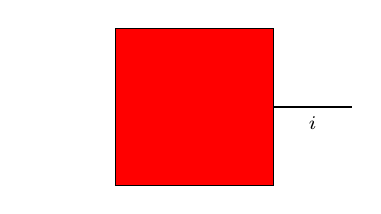
\begin{tikzpicture}
        \draw[fill=red] (0,0) rectangle (2,2) node[pos=0.5]{};
        \draw[](2, 1) -- (3, 1) 
         node[draw=none,fill=none,font=\scriptsize,midway,below]{$i$};
        \draw (-1, 1) node[draw=none]{};
    \end{tikzpicture}
    \caption{rank 1 tensor. Each index is repressented by a line}
    \label{fig:r1t}
\end{figure}

\begin{figure}[H]
    \centering 
    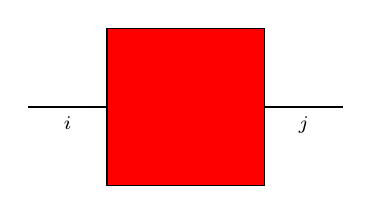
\begin{tikzpicture}
        \draw[fill=red] (0,0) rectangle (2,2) node[pos=0.5]{};
        \draw[](2, 1) -- (3, 1)  
         node[draw=none,fill=none,font=\scriptsize,midway,below]{$j$};
        \draw[](0, 1) -- (-1, 1)  
         node[draw=none,fill=none,font=\scriptsize,midway,below]{$i$};
        
    \end{tikzpicture}
    \caption{rank 2 tensor. Each index is repressented by a line}
    \label{fig:r2t}
\end{figure}

\noindent
Often the indecies are not numbered on these drawing. If we have two tensors we can make them share an index if they have the same dimension, so if we have two rank 3 tensors, one where we have the dimensions of the indexes be 2, 3, 5 and another where it is 1, 4, 3. We can see that they both have an index of size 3 so if we wish we can make them share label for this index. Thus they could have the indecies i, j, k and l, m, j, notice the reuse of j. 

\begin{figure}[H]
    \centering 
    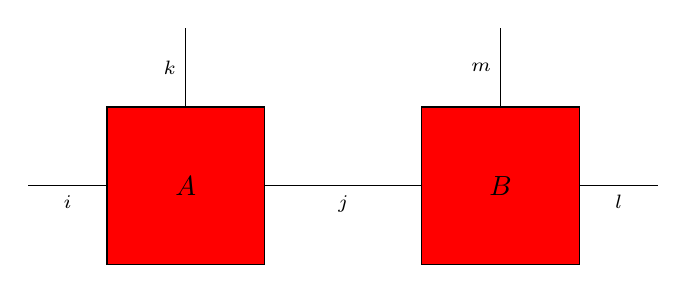
\begin{tikzpicture}
        \draw[fill=red] (0,0) rectangle (2,2) node[pos=0.5]{$A$};
        \draw[](2, 1) -- (3, 1)  
         node[draw=none,fill=none,font=\scriptsize,midway,below]{};
        \draw[](0, 1) -- (-1, 1)  
         node[draw=none,fill=none,font=\scriptsize,midway,below]{$i$};
        \draw[](1, 2) -- (1, 3)  
         node[draw=none,fill=none,font=\scriptsize,midway,left]{$k$};
        
        \draw[fill=red](4,0) rectangle (6,2) node[pos=0.5]{$B$};
        \draw[](6, 1) -- (7, 1)  
         node[draw=none,fill=none,font=\scriptsize,midway,below]{$l$};
        \draw[](4, 1) -- (3, 1)  
         node[draw=none,fill=none,font=\scriptsize,below]{$j$};
        \draw[](5, 2) -- (5, 3)  
         node[draw=none,fill=none,font=\scriptsize,midway,left]{$m$};
    \end{tikzpicture}
    \caption{rank 3 tensors sharing index $j$.}
    \label{fig:2r3t}
\end{figure}

\noindent
But what is this good for? In essence, when we make tensors share indecies it is a way to symbolise that we are multiplying them, matrix multiplication style. The acctual computation of the multiplication can be done at a later point we are just marking our intention. This is important as we might want to build an entire network of tensors and then be strategic about which shared indecies we choose to \textit{contract}. Contracting a shared index is synonumus with computing the product of the two tensors. 
\begin{figure}[H]
    \centering 
    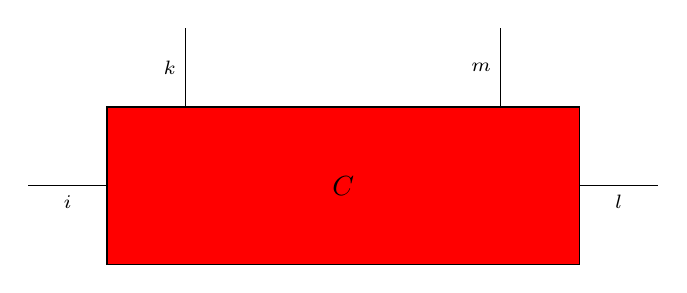
\begin{tikzpicture}
        \draw[fill=red](0,0) rectangle (6,2) node[pos=0.5]{$C$};
        \draw[](0, 1) -- (-1, 1)  
         node[draw=none,fill=none,font=\scriptsize,midway,below]{$i$};
        \draw[](1, 2) -- (1, 3)  
         node[draw=none,fill=none,font=\scriptsize,midway,left]{$k$};
        
        \draw[](6, 1) -- (7, 1)  
         node[draw=none,fill=none,font=\scriptsize,midway,below]{$l$};
        \draw[](5, 2) -- (5, 3)  
         node[draw=none,fill=none,font=\scriptsize,midway,left]{$m$};
    \end{tikzpicture}
    \caption{rank 4 tensor after contracting shared index $j$ from Figure \ref{fig:2r3t}.}
    \label{fig:4t}
\end{figure}
\noindent
in this example we have two tensors A and B where each have elements of the form $a_{ijk}, b_{lmj}$ resulting in a single tensor C with the elements $$c_{iklm}=\displaystyle\sum_{x=0}^{dim(j)-1} a_{ixk}b_{lmx} $$
here $dim(j)=3$ and we subtract 1 since the elements are 0 indexed. In \textit{tensor notation} the summation is implicit if there is a shared index in such an equation so we would just write $c_{iklm}=a_{ijk}b_{lmj}$
